\chapter{Microbiomas y simbiosis}\label{ch:b3:microbiomes}

El cuerpo humano lleva unos treinta y ocho billones de bacterias, más o
menos una por cada célula propia, la mayoría en el último metro del
intestino, donde pesan aproximadamente lo mismo que el encéfalo y llevan
cien veces más genes que él. Un ratón criado sin ninguna de ellas necesita un
tercio más de comida para mantener el peso, tiene un sistema inmunitario
raquítico y se comporta de manera extraña. Una planta de guisante
alimenta con la décima parte de su azúcar a bacterias alojadas en nódulos
de sus raíces y recibe a cambio su nitrógeno; cuatro quintas partes de
todas las plantas terrestres cambian azúcar por fosfato con hongos
envueltos en sus raíces, como llevan haciendo cuatrocientos millones de
años; un coral es un animal que cultiva algas dentro de sus células y que
muere cuando el mar se calienta lo bastante como para que las expulse.
Los seres vivos no son individuos sino consorcios, y este capítulo trata
de la biología de esas asociaciones: cómo se cuentan y se caracterizan
por secuenciación, qué intercambian los socios, cómo se negocia y se
vigila el intercambio y por qué algunos socios acaban como orgánulos.

\section{Palabras para vivir juntos}

\begin{definition}[Simbiosis]\label{def:b3:microbiomes:symbiosis}
\index{simbiosis}\index{mutualismo}\index{comensalismo}\index{holobionte}\index{microbioma}\index{transmisión vertical}
La \emph{simbiosis} es la asociación íntima y sostenida de organismos de
especies distintas; es un \emph{mutualismo} si ganan ambos, un
\emph{comensalismo} si gana uno y el otro no se ve afectado, y un
parasitismo si uno gana a costa del otro --- y una misma pareja puede
desplazarse por esa línea según las circunstancias. Un
\emph{endosimbionte} vive dentro de las células de su hospedador; un
socio \emph{obligado} no puede vivir solo. Los simbiontes se transmiten
\emph{verticalmente}, de padres a hijos (las \emph{Buchnera} del pulgón
pasan por el huevo), u \emph{horizontalmente}, adquiridos de nuevo en
cada generación del ambiente o de otros hospedadores (el \emph{Vibrio}
del calamar, las bacterias del intestino humano). El \emph{microbioma} es
toda la comunidad de microbios de un hábitat --- un intestino, la
superficie de una hoja, un gramo de suelo --- y el \emph{holobionte} es
un hospedador junto con su microbioma, considerado como la unidad que la
selección natural ve.
\end{definition}

\begin{example}[Tres socios obligados]\label{ex:b3:microbiomes:obligate}
La \emph{Buchnera} del pulgón lleva doscientos millones de años viviendo
dentro de las células de su hospedador, fabrica los aminoácidos
esenciales que le faltan a la savia del floema y ha encogido su genoma
hasta \qty{640}{kb} --- una séptima parte del de sus parientes de vida
libre ---, tras perder todos los genes que ahora aporta el hospedador. La
bacteria \emph{Wolbachia}, presente en dos tercios de las especies de
insectos, se transmite solo por los huevos y ha evolucionado por eso para
favorecer a las hembras: mata a los embriones macho, los feminiza o hace
que los huevos de las hembras no infectadas mueran al fecundarlos machos
infectados (la \emph{incompatibilidad citoplasmática}), lo que la propaga
por una población; los mosquitos que la llevan transmiten mal el dengue,
y soltarlos ha reducido el dengue en varias ciudades. La ameba
\emph{Paulinella} acogió hace unos cien millones de años a una
cianobacteria que hoy no es del todo una bacteria ni del todo un
cloroplasto --- un segundo origen independiente de los orgánulos
fotosintéticos, sorprendido a medio camino.
\end{example}

\section{Contar una comunidad}

\begin{method}[Perfilar un microbioma por secuenciación]\label{met:b3:microbiomes:16s}
\index{secuenciación del ARNr 16S}\index{metagenómica}\index{unidad taxonómica operativa}
La mayoría de los microbios no pueden cultivarse; se cuentan por su ADN.
(1) Extráigase el ADN de la muestra --- heces, suelo, agua de mar filtrada
sobre una membrana. (2) O bien amplifíquese el gen del ARN ribosómico de
la subunidad pequeña (el \emph{16S}) con \omterm{def:b3:genetic-engineering:pcr}{cebadores} que casen con sus
regiones universales y secuénciense las regiones variables que hay entre
ellas --- un estudio de \emph{amplicones}, barato, que identifica las
bacterias hasta el género aproximadamente y las cuenta por el número de
lecturas ---; o bien secuénciese todo el ADN --- la \emph{metagenómica de
escopetazo}, que recupera genes y genomas enteros y por tanto informa de
lo que la comunidad puede hacer y no solo de quién está ahí. (3)
Agrúpense las lecturas en variantes de secuencia o en \emph{\omterm{met:b3:microbiomes:16s}{unidades
taxonómicas operativas}} (OTU, convencionalmente al \qty{97}{\%} de
identidad para una ``especie''), asígnense por comparación con bases de
datos (\cref{ch:b3:bioinformatics}) y tabúlense los recuentos por
muestra. (4) Calcúlese la diversidad dentro de una muestra y compárese la
composición entre muestras. Los recuentos son relativos --- las lecturas
de una muestra suman un total fijo --- y los sesgan la extracción, los
\omterm{def:b3:genetic-engineering:pcr}{cebadores} y el número de copias, de modo que las diferencias entre
muestras procesadas igual son fiables allí donde los números absolutos no
lo son.
\end{method}

\begin{definition}[Diversidad]\label{def:b3:microbiomes:diversity}
\index{riqueza de especies}\index{índice de Shannon}\index{índice de Simpson}\index{rarefacción}
Para una comunidad de $S$ especies con abundancias relativas $p_{1},\dots,
p_{S}$ ($\sum p_{i} = 1$): la \emph{riqueza} es $S$; el \emph{índice de
Shannon} $H = -\sum_{i} p_{i}\ln p_{i}$ mide la incertidumbre sobre la
especie de un individuo tomado al azar, y $e^{H}$ es el número de
especies igualmente abundantes que daría la misma incertidumbre (el
número efectivo de especies); el \emph{índice de Simpson}
$D = \sum_{i} p_{i}^{2}$ es la probabilidad de que dos individuos tomados
al azar sean de la misma especie, y $1/D$ es otro número efectivo,
ponderado hacia las especies comunes. La riqueza depende de cuántos
individuos se hayan mirado: una \emph{curva de rarefacción} representa
las especies encontradas frente al número de individuos muestreados, y se
aplana cuando ya se han visto casi todas las especies.
\end{definition}

\begin{theorem}[Rarefacción]\label{thm:b3:microbiomes:rarefaction}
\index{rarefacción!fórmula}\index{cobertura de Good}
Una muestra contiene $N$ individuos de $S$ especies, $N_{i}$ de la
especie $i$. El número esperado de especies en una submuestra aleatoria
de $n$ individuos, tomada sin reposición, es
\[
E[S_{n}] = \sum_{i=1}^{S}\left[1 - \frac{\binom{N - N_{i}}{n}}
{\binom{N}{n}}\right],
\]
que sube con $n$ y vale $S$ en $n = N$. Dos muestras de tamaños distintos
se comparan rarefaciendo ambas al mismo $n$. La fracción de los
individuos de la comunidad que pertenecen a especies aún no vistas se
estima con la \emph{\omterm{thm:b3:microbiomes:rarefaction}{cobertura de Good}}: aproximadamente $f_{1}/N$, donde
$f_{1}$ es el número de especies vistas exactamente una vez (las
singletonas).
\end{theorem}
\begin{proof}
La especie $i$ está ausente de la submuestra exactamente cuando los $n$
individuos se toman de las $N - N_{i}$ restantes, lo que ocurre en
$\binom{N - N_{i}}{n}$ de las $\binom{N}{n}$ submuestras igualmente
probables; de modo que la especie $i$ está presente con probabilidad
$1 - \binom{N-N_{i}}{n}/
\binom{N}{n}$, y el recuento esperado de especies presentes es la suma de
esas probabilidades (la esperanza de una suma de indicadores). Cada
término crece con $n$, y en $n = N$ todo binomio del numerador es cero.
La estimación de Good: un individuo tomado a continuación pertenece a una
especie no vista con aproximadamente la probabilidad de que un individuo
elegido al azar de la muestra fuera el único de su clase, $f_{1}/N$
(Good, 1953); su justificación se admite aquí.
\end{proof}

\begin{example}[Dos intestinos]\label{ex:b3:microbiomes:two-guts}
Una muestra de $1000$ lecturas de una persona da $150$ especies, con
$H = 3.5$ y $40$ singletonas; una muestra de $5000$ lecturas de otra da
$260$ especies. La segunda no es necesariamente más diversa: se muestreó
cinco veces más a fondo, y rarefacerla a $1000$ lecturas puede dar $150$
también. La cobertura de la primera muestra es $1 - 40/1000 =
\qty{96}{\%}$: el cuatro por ciento de las bacterias de ese intestino
pertenece a especies que la muestra no vio nunca, y una muestra más
profunda las encontrará. Los números efectivos, unas $e^{3.5} \approx 33$
especies de uniformidad frente a una riqueza de $150$, dicen que unas
pocas especies dominan --- que es el aspecto que tiene todo intestino.
\end{example}

\begin{omfigure}
\begin{tikzpicture}
\begin{axis}[
  width=0.68\linewidth, height=5.6cm,
  axis x line=bottom, axis y line=left,
  xmin=0, xmax=5000, ymin=0, ymax=300,
  xlabel={lecturas muestreadas, $n$}, ylabel={especies observadas},
  xlabel style={font=\small, at={(axis description cs:0.5,-0.12)}, anchor=north}, ylabel style={font=\small},
  tick label style={font=\small}, xtick={0,1000,2000,3000,4000,5000}, ytick={0,100,150,200,260},
  clip=false,
]
\addplot[very thick, omDef, domain=0:5000, samples=60] {260*(1-exp(-x/1500))};
\addplot[very thick, omThm, domain=0:1000, samples=30] {150*(1-exp(-x/300))*1.0};
\addplot[very thick, omThm, dashed, domain=1000:5000, samples=30] {150*(1-exp(-x/300))*1.0 + 8*(1-exp(-(x-1000)/2000))};
\draw[dashed, gray] (axis cs:1000,0) -- (axis cs:1000,300);
\node[font=\scriptsize, omDef, anchor=north west] at (axis cs:1200,292) {segundo intestino: $260$ especies con $5000$ lecturas};
\node[font=\scriptsize, omThm, anchor=north east] at (axis cs:4900,140) {primer intestino: $150$ con $1000$, cerca de su meseta};
\node[font=\scriptsize, gray, anchor=south west] at (axis cs:1050,10) {rarefacción hasta aquí para comparar};
\end{axis}
\end{tikzpicture}

{\small Curvas de \omterm{def:b3:microbiomes:diversity}{rarefacción}. Las especies encontradas suben con las
lecturas muestreadas y se aplanan a medida que se agota la comunidad; dos
muestras se comparan a la misma profundidad. Aquí el segundo intestino
sigue subiendo con $5000$ lecturas, de modo que su riqueza verdadera es
todavía mayor.}
\end{omfigure}

\section{El microbioma humano}

\begin{definition}[La comunidad del intestino]\label{def:b3:microbiomes:gut}
\index{microbioma intestinal}\index{ácido graso de cadena corta}\index{resistencia a la colonización}\index{disbiosis}
El intestino humano alberga unos $4\times 10^{13}$ bacterias, casi todas
en el colon a $10^{11}$ por gramo de contenido, frente a $10^{3}$ por
gramo en el estómago ácido y de $10^{4}$ a $10^{7}$ a lo largo del
intestino delgado, cuyo flujo es rápido y cuya bilis es hostil. Hay de
quinientas a mil especies por persona, en su mayoría de dos filos, los
Bacteroidetes y los Firmicutes, y casi todas anaerobias; el conjunto de
cada persona es distinto y estable durante años, fijado en gran medida en
los tres primeros años de vida a partir de la madre y del hogar. Lo que
hacen: fermentan la fibra que las enzimas humanas no pueden digerir en
\emph{ácidos grasos de cadena corta} --- acetato, propionato, butirato
---, que alimentan a las propias células del colon y aportan hasta la
décima parte de las calorías del hospedador; fabrican vitamina~K y
algunas vitaminas del grupo B; transforman ácidos biliares y fármacos;
ocupan todos los nichos, de modo que un invasor no encuentra asidero (la
\emph{resistencia a la colonización}); y entrenan al sistema inmunitario,
cuyos linfocitos~T reguladores y células secretoras de IgA se desarrollan
en respuesta a ellas (\cref{ch:b3:adaptive-immunity}). Una comunidad
desplazada de ese estado --- menos especies, menos fermentadoras, más
aerobias facultativas --- es una \emph{disbiosis}, que se ve en la
enfermedad inflamatoria intestinal, después de los \omterm{def:b3:bacteriology:antibiotics}{antibióticos} y en la
obesidad, aunque cuál es la causa y cuál el efecto suele estar poco
claro.
\end{definition}

\begin{proof}[Evidencia]
Los ratones criados libres de gérmenes en aisladores estériles (Gordon y
colaboradores, años dos mil) tienen paredes intestinales finas, órganos
linfoides pequeños y niveles bajos de anticuerpos, y necesitan un
\qty{30}{\%} más de calorías para mantener el peso; colonizados con una
microbiota normal de ratón ganan grasa en dos semanas. Al recibir la
microbiota de un ratón obeso en lugar de la de uno delgado, los ratones
libres de gérmenes ganaron más grasa con la misma comida (Turnbaugh,
2006): la propia comunidad afecta a la cosecha de energía. En el ser
humano, la colitis recurrente por \emph{Clostridioides difficile} --- una
\omterm{def:b3:microbiomes:gut}{disbiosis} en la que los \omterm{def:b3:bacteriology:antibiotics}{antibióticos} han eliminado a los competidores de
un formador de esporas productor de toxinas --- se curó en el
\qty{94}{\%} de los pacientes con una infusión de heces de un donante
sano, frente al \qty{31}{\%} con el \omterm{def:b3:bacteriology:antibiotics}{antibiótico} habitual (van~Nood,
2013), el primer ensayo aleatorizado en el que el fármaco era una
comunidad y no una molécula.
\end{proof}

\begin{omfigure}
\begin{tikzpicture}
\begin{axis}[
  width=0.68\linewidth, height=5.4cm,
  ybar, bar width=18pt,
  axis x line=bottom, axis y line=left,
  ymode=log, ymin=1, ymax=1e13,
  symbolic x coords={estomago, duodeno, yeyuno, ileon, colon},
  xticklabels={estómago, duodeno, yeyuno, íleon, colon},
  xtick=data, ytick={1e1,1e3,1e5,1e7,1e9,1e11},
  ylabel={bacterias por gramo de contenido},
  ylabel style={font=\small}, tick label style={font=\small},
  clip=false,
]
\addplot[fill=omDef!40, draw=omDef] coordinates {(estomago,1e3) (duodeno,1e4) (yeyuno,1e5) (ileon,1e7) (colon,1e11)};
\node[font=\scriptsize, anchor=west, xshift=10pt] at (axis cs:estomago,3e3) {ácido, pH 2};
\node[font=\scriptsize, anchor=south] at (axis cs:yeyuno,1.5e5) {bilis, flujo rápido};
\node[font=\scriptsize, anchor=south, align=center] at (axis cs:colon,1.5e11) {lento, anaerobio:\\el fermentador};
\end{axis}
\end{tikzpicture}

{\small Densidad bacteriana a lo largo del intestino humano, en escala
logarítmica: una subida de cien millones de veces desde el estómago ácido
hasta el colon, donde vive casi la totalidad de los microbios del cuerpo.}
\end{omfigure}

\begin{omfigure}
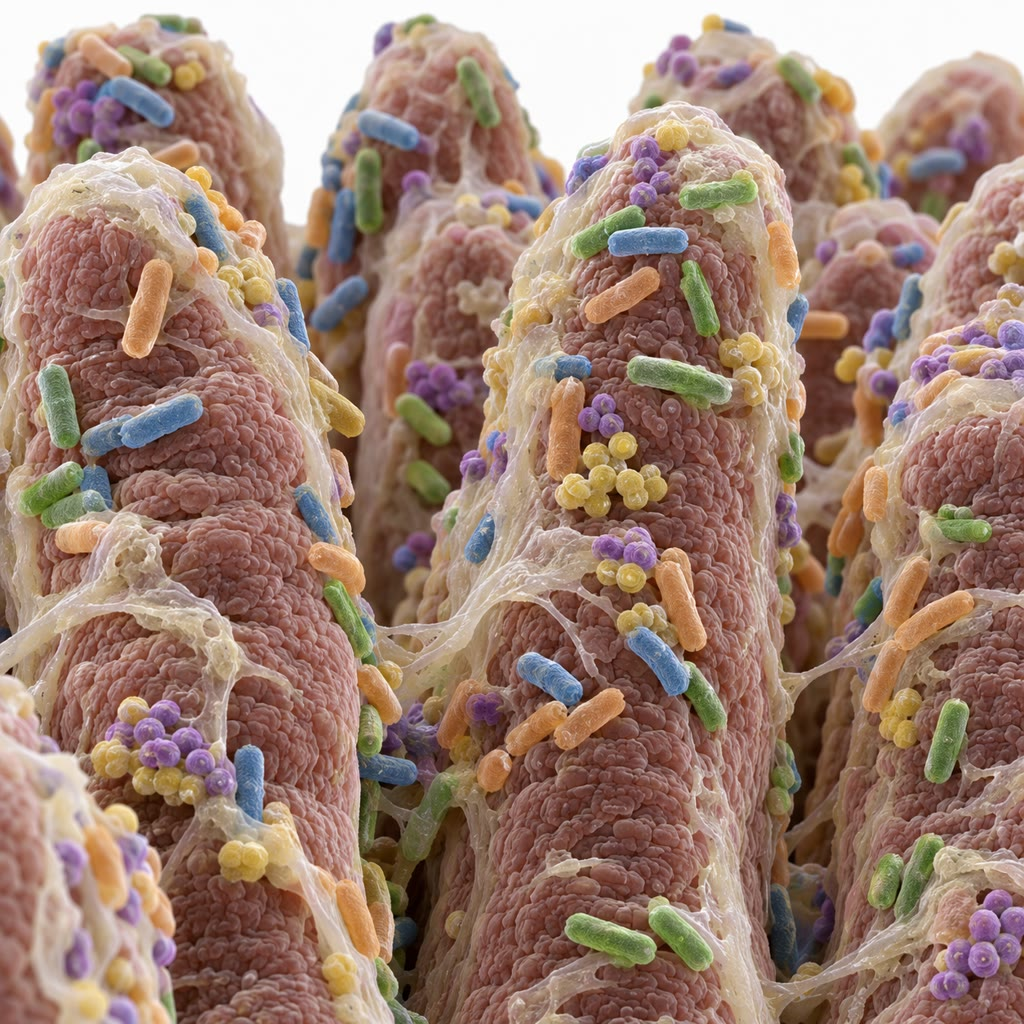
\includegraphics[width=0.40\linewidth]{images/book5/ai/b5-14-gut-microbiota.jpg}

{\small La superficie del revestimiento intestinal en el microscopio
electrónico de barrido, con bacterias de varias clases alojadas en el
moco entre las vellosidades.}
\end{omfigure}

\section{Las plantas y sus socios}

\begin{definition}[La simbiosis entre leguminosa y rizobio]\label{def:b3:microbiomes:nodule}
\index{rizobios}\index{nódulo radicular}\index{factor Nod}\index{leghemoglobina}\index{nitrogenasa}
Las leguminosas alojan bacterias fijadoras de nitrógeno (los
\emph{rizobios}) en \emph{nódulos radiculares}, órganos construidos a tal
efecto tras un diálogo molecular. La raíz secreta flavonoides; un rizobio
de la especie adecuada responde con \emph{factores Nod} ---
lipoquitooligosacáridos cuyos adornos especifican al socio ---; un
receptor quinasa del pelo radicular los une y desencadena oscilaciones de
calcio en el núcleo, el enroscamiento del pelo radicular alrededor de las
bacterias y un \emph{cordón de infección} que crece hacia dentro por las
células mientras la corteza de debajo empieza a dividirse formando un
nódulo. Las bacterias se liberan dentro de las células del nódulo
envueltas en membranas y se diferencian en \emph{bacteroides} que
expresan la \emph{nitrogenasa}, la enzima que reduce el N$_{2}$ a amoníaco
a un coste de dieciséis ATP por molécula. El oxígeno destruye la
nitrogenasa, y sin embargo los bacteroides respiran con fuerza; el nódulo
resuelve la contradicción con una barrera de difusión y con la
\emph{leghemoglobina}, una hemoglobina vegetal que une el oxígeno con
fuerza y se lo lleva a los bacteroides a baja concentración libre --- es
lo que hace rosado un nódulo cortado. La planta paga entre el seis y el
diez por ciento de su fotosintato y recibe casi todo su nitrógeno; el
nitrógeno fijado por las leguminosas cultivadas del mundo se acerca al de
la industria de los fertilizantes.
\end{definition}

\begin{omfigure}
\begin{tikzpicture}[every node/.style={font=\scriptsize}, >=stealth]
  % stage 1: root hair and bacteria, flavonoid / Nod factor exchange
  \begin{scope}
    \draw[thick, omMeth!60!black, fill=omMeth!15] (0,0) rectangle (1.2,3.0);
    \draw[thick, omMeth!60!black, fill=omMeth!15] (1.2,1.6) .. controls (2.4,1.7) and (2.6,2.6) .. (2.9,2.4) .. controls (2.5,2.3) and (2.3,1.4) .. (1.2,1.2) -- cycle;
    \foreach \p in {(3.1,2.7),(3.4,2.3),(3.3,1.9)} \fill[omProp] \p ellipse (0.14 and 0.07);
    \draw[->, omMeth!60!black, thick] (2.6,1.5) -- (3.2,1.4); \node[below, omMeth!60!black] at (3.0,1.35) {flavonoides};
    \draw[<-, omProp, thick] (2.5,2.85) -- (3.0,3.0); \node[above, omProp] at (2.4,2.95) {factores Nod};
    \node[below, align=center] at (1.6,-0.2) {1. diálogo: pelo radicular\\y rizobios};
  \end{scope}
  % stage 2: curled hair, infection thread
  \begin{scope}[xshift=4.6cm]
    \draw[thick, omMeth!60!black, fill=omMeth!15] (0,0) rectangle (1.2,3.0);
    \draw[thick, omMeth!60!black, fill=omMeth!15] (1.2,1.6) .. controls (2.3,1.8) and (2.8,2.6) .. (2.2,2.8) .. controls (1.9,2.9) and (1.8,2.5) .. (2.0,2.4) .. controls (2.3,2.2) and (1.9,1.3) .. (1.2,1.2) -- cycle;
    \draw[omProp, very thick] (2.05,2.55) .. controls (1.8,2.1) and (1.4,1.7) .. (0.4,1.3);
    \foreach \p in {(1.85,2.3),(1.5,1.9),(1.1,1.6),(0.7,1.4)} \fill[omProp] \p ellipse (0.1 and 0.05);
    \node[right, omProp, font=\tiny] at (2.3,1.0) {cordón de infección};
    \foreach \p in {(0.3,0.5),(0.6,0.7),(0.9,0.5)} \draw[omMeth!60!black] \p circle (0.12);
    \node[below, align=center] at (1.6,-0.2) {2. el pelo se enrosca; el cordón entra;\\las células de la corteza se dividen};
  \end{scope}
  % stage 3: nodule
  \begin{scope}[xshift=9.0cm]
    \draw[thick, omMeth!60!black, fill=omMeth!15] (0,0) rectangle (1.2,3.0);
    \draw[thick, omThm!60!black, fill=omThm!25] (1.2,1.5) ellipse (1.3 and 1.0);
    \foreach \p in {(1.0,1.5),(1.5,1.8),(1.6,1.2),(1.1,1.9),(1.2,1.1),(2.0,1.5)} \fill[omProp] \p circle (0.1);
    \node[right, align=left] at (2.6,2.0) {nódulo: bacteroides\\con nitrogenasa};
    \node[right, align=left, omThm!60!black] at (2.6,1.1) {rosado: la leghemoglobina\\mantiene bajo el O$_2$};
    \draw[->, thick] (0.6,2.4) -- (1.0,2.0) node[pos=0, above] {azúcar};
    \draw[<-, thick] (0.6,0.6) -- (1.0,1.0) node[pos=0, below] {NH$_3$};
    \node[below, align=center] at (1.6,-0.2) {3. los bacteroides fijan N$_2$;\\azúcar por amoníaco};
  \end{scope}
\end{tikzpicture}

{\small Cómo se hace un nódulo. Los flavonoides de la raíz y los \omterm{def:b3:microbiomes:nodule}{factores
Nod} del rizobio identifican a los socios; el pelo radicular se enrosca,
un cordón de infección lleva las bacterias hacia dentro y la corteza
construye un nódulo en el que los bacteroides, mantenidos a bajo oxígeno
por la \omterm{def:b3:microbiomes:nodule}{leghemoglobina}, fijan nitrógeno a cambio de azúcar.}
\end{omfigure}

\begin{definition}[Micorrizas]\label{def:b3:microbiomes:mycorrhiza}
\index{micorriza}\index{micorriza arbuscular}\index{vía común de la simbiosis}
Las \emph{micorrizas} son asociaciones de raíces con hongos, presentes en
cerca del \qty{80}{\%} de las especies vegetales y en los fósiles de
plantas terrestres más antiguos. En las \emph{micorrizas arbusculares} el
hongo entra en las células de la raíz y se ramifica en un arbúsculo con
forma de árbol a través del cual pasan a la planta fosfato, nitrógeno y
agua, y al hongo azúcares y lípidos; las hifas del hongo multiplican por
cien la superficie absorbente de la raíz y alcanzan fosfato al que la
raíz no llega. En las \emph{ectomicorrizas}, propias de los árboles de
bosque, el hongo envaina la raíz y crece entre las células. Los genes
vegetales que admiten al hongo son la misma \emph{vía común de la
\omterm{def:b3:microbiomes:symbiosis}{simbiosis}} --- receptor, picos de calcio, factores de transcripción ---
que las leguminosas reutilizan para los \omterm{def:b3:microbiomes:nodule}{rizobios}: el nódulo es un invento
tardío construido sobre una asociación con hongos cuatrocientos millones
de años más antigua.
\end{definition}

\begin{proposition}[El comercio y su vigilancia]\label{prop:b3:microbiomes:sanctions}
\index{elección de socio}\index{sanciones}\index{tramposo}
Un \omterm{def:b3:microbiomes:symbiosis}{mutualismo} es un intercambio, y cada socio está seleccionado para dar
menos y tomar más; persiste porque el otro socio puede tomar represalias.
Las leguminosas restringen el oxígeno a los nódulos cuyos \omterm{def:b3:microbiomes:nodule}{rizobios} no
fijan nitrógeno y reducen a la mitad su reproducción (Kiers, 2003): son
\emph{sanciones}. Las plantas de las redes micorrícicas asignan más
carbono a los hongos que entregan más fosfato, y los hongos más fosfato a
las raíces que pagan más carbono --- un mercado en el que ambas partes
premian al mejor comerciante (Kiers, 2011). Los calamares expulsan a las
bacterias del órgano luminoso que no brillan; el sistema inmunitario
humano tolera a las comensales que se quedan en la luz y ataca a las que
cruzan la pared. Cuando un hospedador no puede ni elegir ni sancionar ---
un endosimbionte heredado por el huevo ---, la alineación de intereses
viene en cambio de un destino compartido: un simbionte de \omterm{def:b3:microbiomes:symbiosis}{transmisión
vertical} se reproduce solo cuando lo hace su hospedador, y la selección
sobre el simbionte favorece la reproducción del hospedador. El modo de
transmisión predice así el carácter de la asociación: la \omterm{def:b3:microbiomes:symbiosis}{transmisión
vertical} hacia el \omterm{def:b3:microbiomes:symbiosis}{mutualismo} y la dependencia, y la horizontal hacia una
explotación contenida por la vigilancia.
\end{proposition}
\admitted

\begin{omfigure}
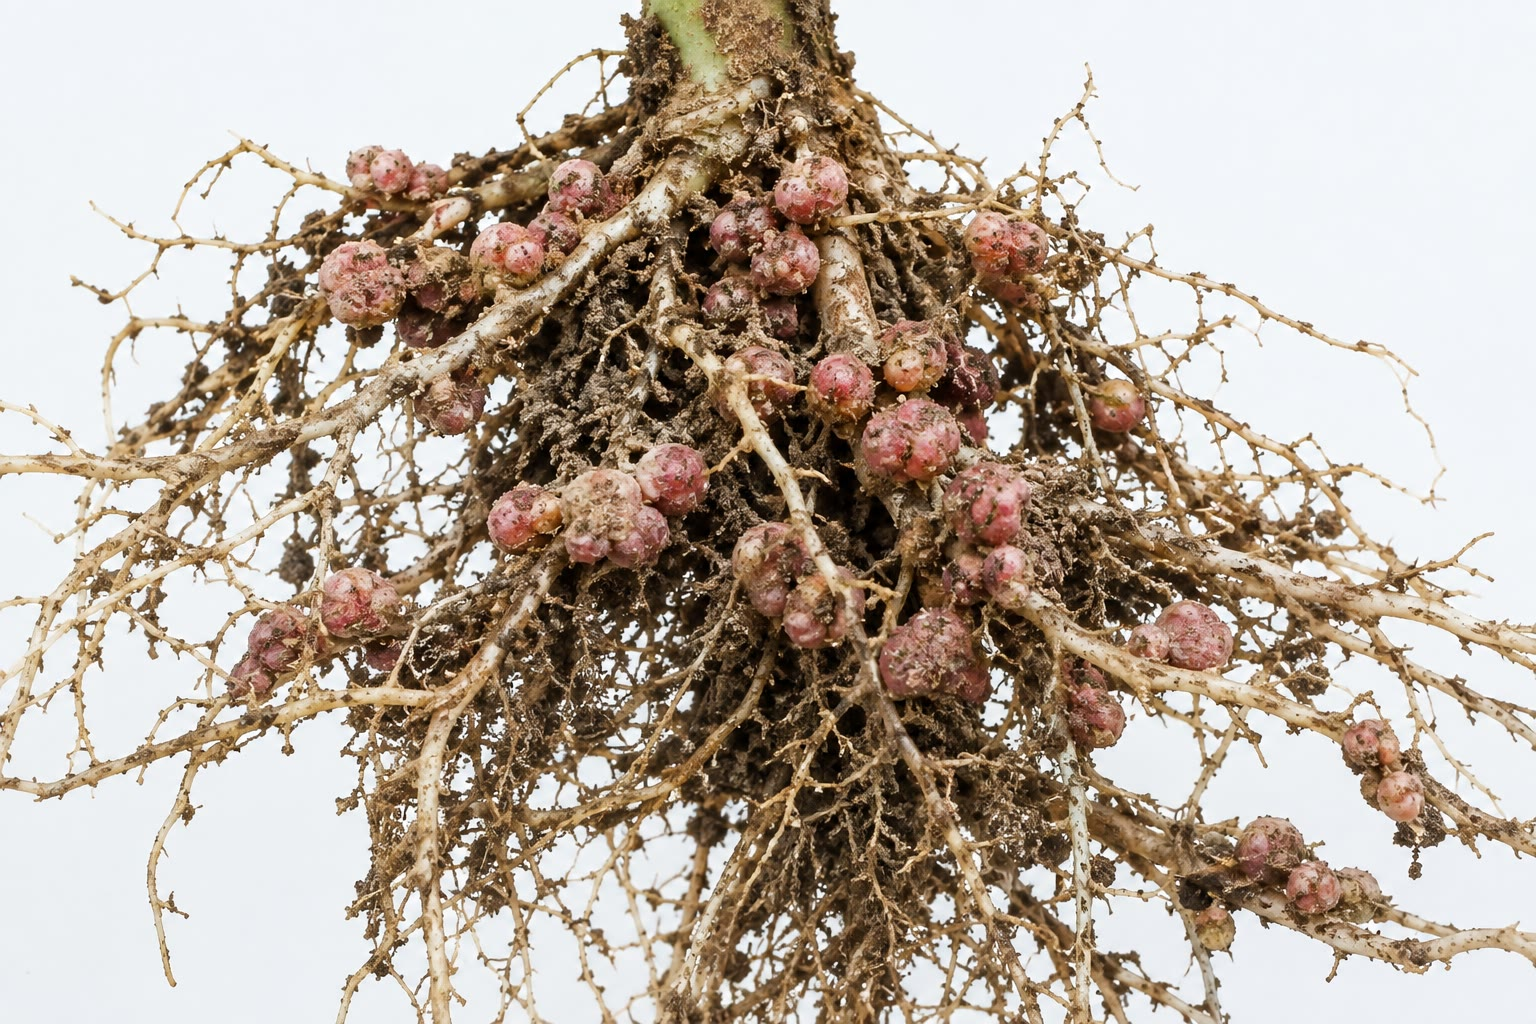
\includegraphics[width=0.46\linewidth]{images/book5/ai/b5-14-root-nodules.jpg}\hspace{0.04\linewidth}
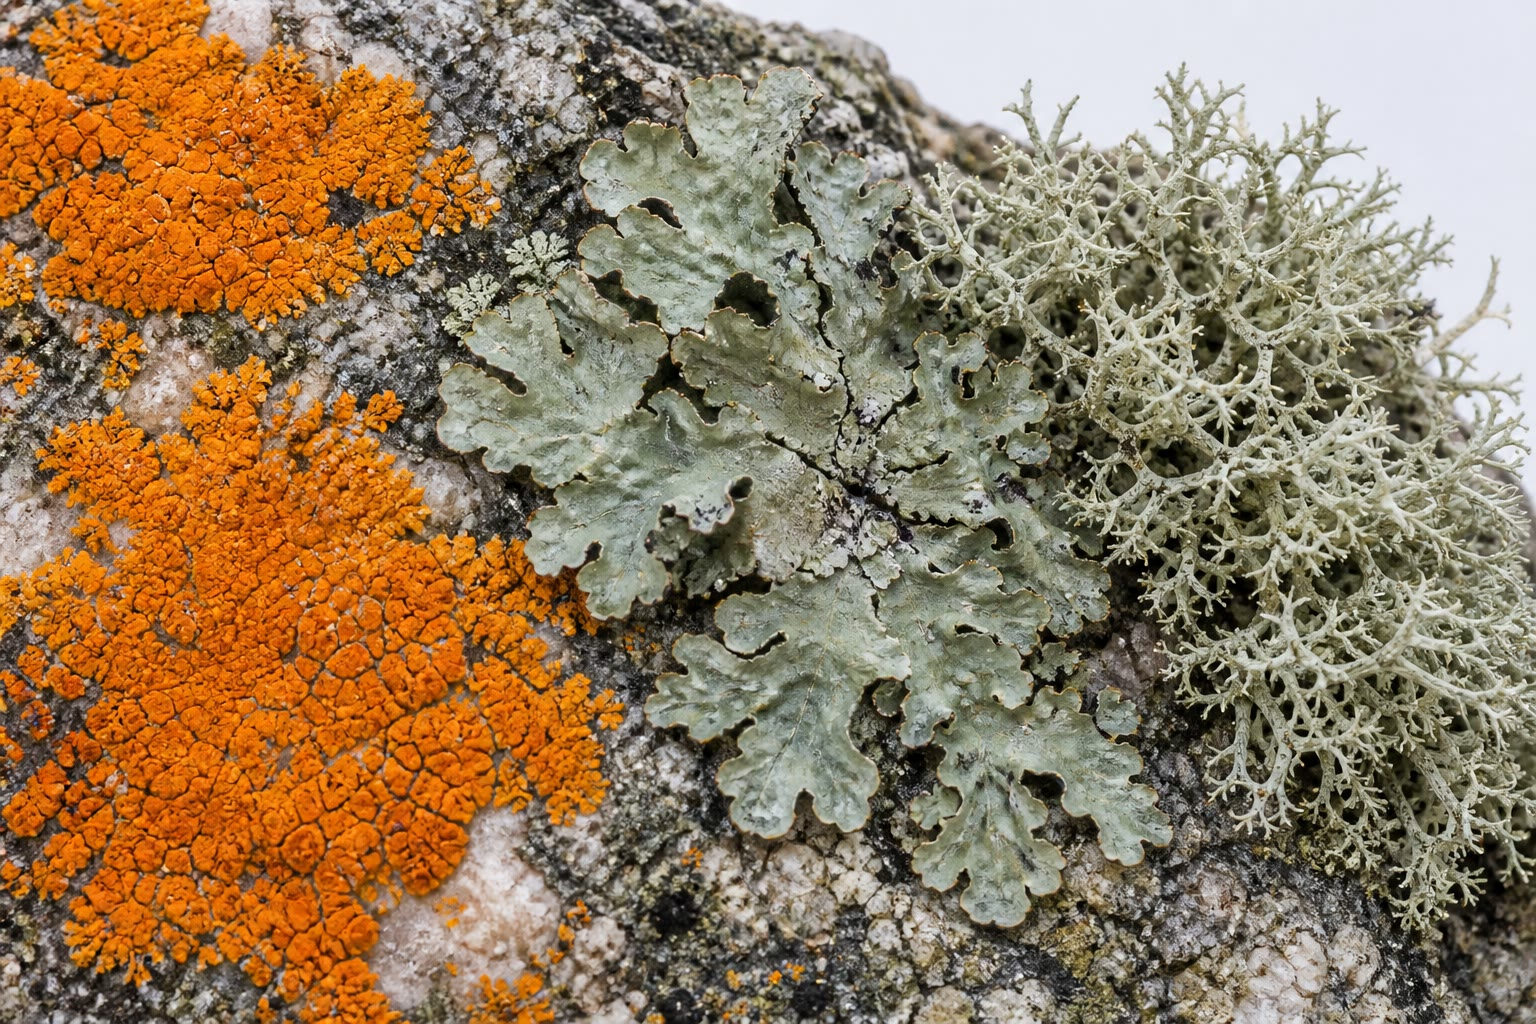
\includegraphics[width=0.46\linewidth]{images/book5/ai/b5-14-lichen.jpg}

{\small Izquierda: las raíces nodulizadas de una leguminosa, con cada
nódulo rosado una fábrica de nitrógeno de bacteroides alimentados con
azúcar. Derecha: líquenes sobre roca --- cada uno un hongo que aloja un
alga fotosintética o una cianobacteria, colonizando juntos una superficie
que ninguno de los dos podría ocupar solo.}
\end{omfigure}

\section{Asociaciones en el mar y en otros sitios}

\begin{definition}[Coral y alga]\label{def:b3:microbiomes:coral}
\index{simbiosis del coral}\index{zooxantelas}\index{blanqueamiento del coral}
Los corales constructores de arrecife alojan algas dinoflageladas (las
\emph{Symbiodiniaceae}, las \emph{zooxantelas}) dentro de las células del
revestimiento de su cavidad digestiva, un millón o más por centímetro
cuadrado. Las algas hacen la fotosíntesis en el tejido del animal, usando
el CO$_{2}$, el amoníaco y el fosfato de desecho del animal, y le
devuelven hasta el \qty{90}{\%} de su carbono fijado en forma de
glicerol, azúcares y aminoácidos, que alimentan al coral y a la
calcificación que construye el arrecife; el coral, a su vez, controla el
suministro de nitrógeno de las algas y con ello su crecimiento. La
asociación funciona dentro de una ventana térmica estrecha: cuando el
agua se mantiene uno o dos grados por encima del máximo de verano durante
unas semanas, la fotosíntesis de las algas se daña, estas liberan oxígeno
reactivo en las células del hospedador y el coral las expulsa --- el
\emph{blanqueamiento}, con el esqueleto blanco asomando a través del
animal translúcido. Un coral blanqueado pasa hambre; se recupera si el
agua se enfría en unas semanas y muere si no. La frecuencia del
blanqueamiento se ha quintuplicado desde 1980, y es el mecanismo por el
que el calentamiento está eliminando los arrecifes.
\end{definition}

\begin{example}[Simbiosis que construyen hábitats]\label{ex:b3:microbiomes:habitats}
Un \emph{liquen} es un hongo que aloja un alga verde o una
cianobacteria, con el hongo aportando estructura, retención de agua y
minerales disueltos de la roca, y el fotobionte aportando azúcar (y, si
es una cianobacteria, nitrógeno); los líquenes cubren cerca del
\qty{8}{\%} de la superficie terrestre, colonizan la roca desnuda y
empiezan a convertirla en suelo. El gusano tubícola \emph{Riftia} de las
fuentes hidrotermales profundas no tiene boca ni intestino de adulto;
aloja bacterias oxidadoras de sulfuro en un trofosoma y les entrega
sulfuro y oxígeno sobre una hemoglobina que une los dos, y crece más de
un metro al año en la oscuridad con energía química. Las termitas
digieren madera con una comunidad intestinal de protistas y bacterias, y
los rumiantes digieren hierba con un rumen del tamaño de una bañera en el
que bacterias, arqueas y hongos fermentan celulosa a ácidos grasos y
metano; la vaca vive de los ácidos grasos y de los cuerpos de los propios
microbios. En todos los casos una capacidad metabólica --- fotosíntesis,
fijación de nitrógeno, oxidación de sulfuro, digestión de celulosa ---
que el linaje del hospedador nunca desarrolló se ha adquirido de una sola
vez por asociación.
\end{example}

\begin{omfigure}
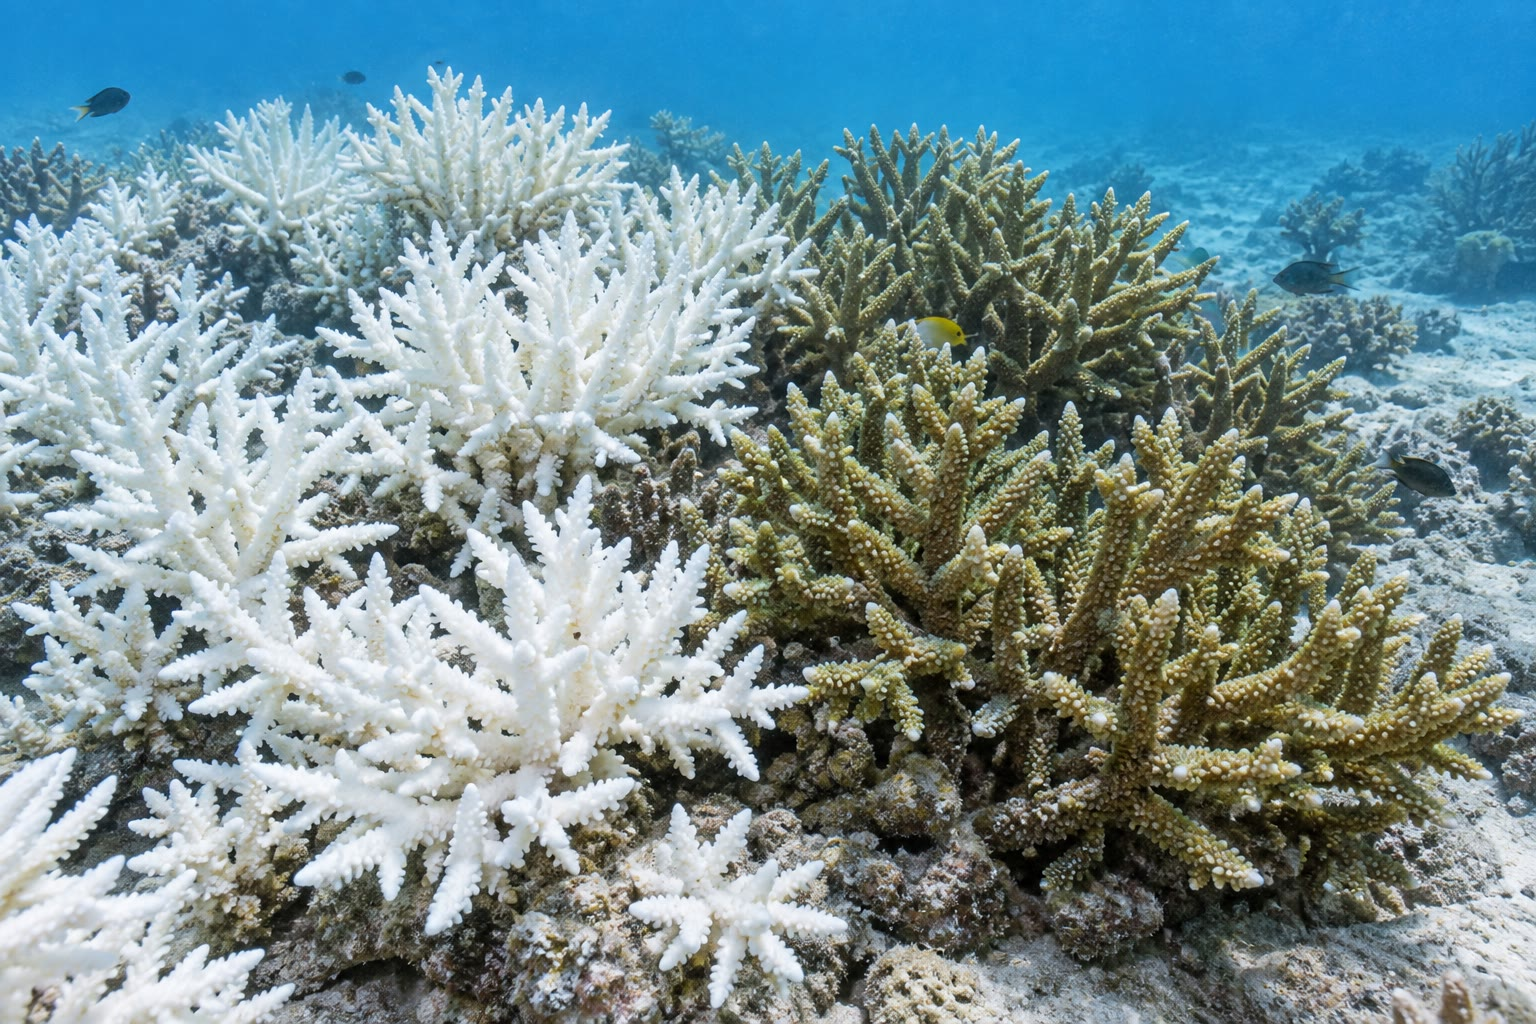
\includegraphics[width=0.56\linewidth]{images/book5/ai/b5-14-coral-bleaching.jpg}

{\small Un arrecife blanqueado a medias: las colonias blancas han
expulsado sus algas tras semanas de agua demasiado cálida; las pardas aún
conservan las suyas. El coral blanco está vivo y hambriento, y tiene unas
semanas para que lo recolonicen.}
\end{omfigure}

\begin{omfigure}
\begin{tikzpicture}[every node/.style={font=\scriptsize}, >=stealth]
  % coral cell with alga
  \draw[very thick, omDef, fill=omDef!8] (0,0) ellipse (3.2 and 2.0); \node[above] at (0,2.05) {célula del coral (gastrodermis)};
  \draw[thick, omMeth!70!black, fill=omMeth!30] (-0.4,-0.1) circle (1.05); \node[align=center] at (-0.4,-0.1) {alga\\(zooxantela)};
  % exchanges
  \draw[->, thick, omMeth!70!black] (0.5,0.4) -- (1.9,0.9) node[right, align=left] {glicerol, azúcares, aminoácidos:\\hasta el \qty{90}{\%} del carbono fijado};
  \draw[<-, thick, omThm] (0.5,-0.5) -- (1.9,-1.0) node[right, align=left] {CO$_2$, NH$_3$, fosfato\\(los desechos del animal)};
  \draw[<-, thick, omProp] (-1.3,0.3) -- (-2.6,1.0) node[left, align=right] {luz a través\\del tejido};
  \node[below, align=center] at (1.5,-2.1) {estrés: agua cálida durante semanas $\to$ fotosíntesis dañada,\\oxígeno reactivo $\to$ alga expulsada $\to$ blanqueamiento};
  % thermometer-like bar on the right
  \begin{scope}[xshift=7.6cm, yshift=-1.6cm]
    \draw[thick] (0,0) rectangle (0.5,3.2);
    \fill[omDef!40] (0,0) rectangle (0.5,2.0); \fill[omProp!60] (0,2.0) rectangle (0.5,2.6); \fill[omThm!60] (0,2.6) rectangle (0.5,3.2);
    \node[right] at (0.6,1.0) {intervalo normal}; \node[right] at (0.6,2.3) {$+\qty{1}{\celsius}$: estrés}; \node[right, align=left] at (0.6,2.9) {$+\qty{2}{\celsius}$ durante semanas:\\blanqueamiento};
    \node[below, align=center] at (0.25,-0.1) {temperatura estival\\del mar};
  \end{scope}
\end{tikzpicture}

{\small El intercambio entre coral y alga: el alga fija carbono con los
desechos del animal y la luz que atraviesa su tejido y devuelve casi todo
como alimento; una subida pequeña y sostenida de la temperatura rompe la
asociación.}
\end{omfigure}

\section{De socio a orgánulo}

\begin{proposition}[La reducción del genoma y el camino hacia el orgánulo]\label{prop:b3:microbiomes:reduction}
\index{reducción del genoma}\index{transferencia génica endosimbiótica}
Un endosimbionte heredado por el huevo vive en una población de unas
pocas células que nunca recombinan con extraños. La selección sobre él es
débil (\cref{ch:b3:molecular-evolution}: una población pequeña fija por
deriva mutaciones levemente dañinas), los genes cuyos productos aporta el
hospedador no se echan de menos cuando se estropean, y un gen perdido no
se recupera nunca. El genoma se encoge por tanto generación tras
generación --- \emph{Buchnera} hasta \qty{640}{kb}, algunos simbiontes de
insectos hasta \qty{140}{kb} y unos pocos centenares de genes, la
mitocondria hasta \qty{16}{kb} y trece proteínas en el ser humano --- y
el núcleo del hospedador adquiere copias de genes del simbionte por
\emph{\omterm{prop:b3:microbiomes:reduction}{transferencia génica endosimbiótica}}, cuyos productos se importan
de vuelta con una secuencia de direccionamiento. Cuando el hospedador
fabrica la mayoría de las proteínas del simbionte, controla su división y
no puede vivir sin él, el simbionte se ha convertido en un orgánulo. Las
mitocondrias y los plastos recorrieron este camino hace dos mil y mil
millones de años (el volumen de primer año); el cromatóforo de
\emph{Paulinella} es un tercer viajero, con cien millones de años de
recorrido.
\end{proposition}

\begin{remark}[El individuo, revisitado]\label{rem:b3:microbiomes:individual}
Un animal o una planta es una comunidad con un genoma en su centro, y la
mayor parte de su repertorio metabólico, y buena parte de su desarrollo y
de su inmunidad, dependen de socios que no heredó en su propio ADN. Las
consecuencias prácticas ya están aquí: el \omterm{def:b3:microbiomes:symbiosis}{microbioma} como fármaco (el
trasplante fecal), como diana de fármacos (el daño colateral de los
\omterm{def:b3:bacteriology:antibiotics}{antibióticos}, la fibra alimentaria como receta), como prueba diagnóstica
y como vía --- mediante simbiontes modificados y mosquitos portadores de
\emph{Wolbachia} --- para cambiar la biología de poblaciones silvestres.
La consecuencia teórica es que la selección natural actúa sobre
asociaciones, y que las asociaciones más fuertes son aquellas en las que
el destino de un socio es el del otro.
\end{remark}

\section{Ejercicios}

\begin{exercise}[$\star$]\label{exo:b3:microbiomes:1}
Defínanse el \omterm{def:b3:microbiomes:symbiosis}{mutualismo}, el \omterm{def:b3:microbiomes:symbiosis}{comensalismo} y el parasitismo, y dese un
ejemplo de cada uno de este capítulo. ¿Por qué una misma pareja de
especies puede moverse entre las categorías?
\end{exercise}

\begin{exercise}[$\star$]\label{exo:b3:microbiomes:2}
Calcúlense $H$, $e^{H}$, $D$ y $1/D$ para una comunidad con abundancias
$0.5$, $0.3$, $0.1$, $0.05$, $0.05$.
\end{exercise}

\begin{exercise}[$\star$]\label{exo:b3:microbiomes:3}
Contrástese un estudio de amplicones del 16S con la metagenómica de
escopetazo: ¿qué informa cada uno, y qué no puede decirnos cada uno?
\end{exercise}

\begin{exercise}[$\star$]\label{exo:b3:microbiomes:4}
Enumérense cuatro servicios que el \omterm{def:b3:microbiomes:gut}{microbioma intestinal} presta a su
hospedador y una enfermedad que sigue a su alteración.
\end{exercise}

\begin{exercise}[$\star\star$]\label{exo:b3:microbiomes:5}
Una muestra de $N = 20$ lecturas contiene especies con
$N_{i} = 10, 6, 3, 1$. Calcúlese $E[S_{n}]$ para $n = 5$ con el teorema,
y la \omterm{thm:b3:microbiomes:rarefaction}{cobertura de Good}.
\end{exercise}

\begin{exercise}[$\star\star$]\label{exo:b3:microbiomes:6}
El colon contiene \qty{400}{g} de contenido a $10^{11}$ bacterias por
gramo; una bacteria pesa \qty{1}{pg} y su genoma tiene \num{4000} genes;
el intestino de una persona tiene $1000$ especies. Estímense la masa del
\omterm{def:b3:microbiomes:symbiosis}{microbioma} y el número de genes distintos que lleva, y compárense con los
\num{20000} del genoma humano.
\end{exercise}

\begin{exercise}[$\star\star$]\label{exo:b3:microbiomes:7}
Explíquese la paradoja del oxígeno del nódulo y cómo la resuelven la
\omterm{def:b3:microbiomes:nodule}{leghemoglobina} y la barrera de difusión. ¿Por qué es rosado un nódulo, y
qué significa un nódulo verde?
\end{exercise}

\begin{exercise}[$\star\star$]\label{exo:b3:microbiomes:8}
Un mutante de leguminosa carece del componente de los picos de calcio de
la \omterm{def:b3:microbiomes:mycorrhiza}{vía común de la simbiosis}. Predíganse su nodulación y su
micorrización, y explíquese qué dice eso sobre la evolución de las dos
\omterm{def:b3:microbiomes:symbiosis}{simbiosis}.
\end{exercise}

\begin{exercise}[$\star\star$]\label{exo:b3:microbiomes:9}
Descríbase el experimento de sanciones de Kiers y qué se predeciría si la
planta no pudiera distinguir los nódulos que fijan de los que no.
\end{exercise}

\begin{exercise}[$\star\star\star$]\label{exo:b3:microbiomes:10}
Demuéstrese que el $E[S_{n}]$ del teorema de la \omterm{def:b3:microbiomes:diversity}{rarefacción} es una
función creciente de $n$ y alcanza $S$ en $n = N$, y muéstrese que para
una especie con $N_{i} \ll N$ y $n \ll N$ su probabilidad de ser vista es
aproximadamente $1 - (1 - n/N)^{N_{i}}$.
\end{exercise}

\begin{exercise}[$\star\star\star$]\label{exo:b3:microbiomes:11}
\emph{Wolbachia} se transmite solo por los huevos. Explíquese por qué la
selección sobre ella favorece a los hospedadores hembra, descríbase la
incompatibilidad citoplasmática y muéstrese por qué permite que una cepa
infectada se propague aunque la infección tenga un pequeño coste.
\end{exercise}

\begin{exercise}[$\star\star\star$]\label{exo:b3:microbiomes:12}
Con la \cref{prop:b3:microbiomes:reduction}, explíquese por qué se encogen
los genomas de los endosimbiontes de \omterm{def:b3:microbiomes:symbiosis}{transmisión vertical} y no los de sus
parientes de vida libre, qué genes se pierden primero y cuáles los
últimos, y qué invertiría la tendencia.
\end{exercise}

\section{Problema: el censo de un intestino}

\begin{problem}[{Problema de fin de semana --- un microbioma intestinal
contado en células, genes y calorías, su diversidad medida y rarefacida,
el balance de nitrógeno de una leguminosa comparado con su azúcar y el
carbono de un arrecife contabilizado, hasta llegar a las calorías que
gana un microbioma, a la cobertura de una muestra de secuenciación y al
azúcar que paga por su nitrógeno un campo de judías}]
\label{pb:b3:microbiomes:1}
Datos: contenido del colon, \qty{400}{g} a $10^{11}$ bacterias por gramo,
con una masa celular de \qty{1}{pg}; $1000$ especies, con \num{4000}
genes cada una y un \qty{30}{\%} de genes compartidos entre dos especies
cualesquiera. Dieta: \qty{30}{g} de fibra al día, fermentada a \omterm{def:b3:microbiomes:gut}{ácidos
grasos de cadena corta} a \qty{10}{mmol} por gramo, cada uno de un valor
de \qty{0.9}{kJ}; una dieta de \qty{9000}{kJ}. Una muestra de
secuenciación: $N = 2000$ lecturas, $S = 180$ especies, $f_{1} = 60$
singletonas; abundancias de las tres especies principales, $0.30$, $0.20$
y $0.10$, y el resto repartido por igual. Un cultivo de judías fija
\qty{150}{kg} de N por hectárea y temporada y paga \qty{8}{g} de azúcar
por gramo de N fijado; su fotosíntesis rinde \qty{12}{t} de azúcar por
hectárea y temporada. \omterm{def:b3:microbiomes:nodule}{Nitrogenasa}: $16$ ATP por N$_{2}$. Un coral:
$10^{6}$ algas por cm$^{2}$, cada una fijando \qty{20}{pg} de carbono al
día, con el \qty{90}{\%} pasado al hospedador; el tejido del coral
respira \qty{15}{\micro g} de carbono por cm$^{2}$ y día.

\medskip
\noindent\textbf{Parte I --- Células y genes.}
\begin{enumerate}
  \item ¿Cuántas bacterias hay en el colon, y cuánto pesan?
  \item ¿A cuántos genomas bacterianos de ADN equivale eso, y cómo se
        compara el total con el ADN de los $3\times 10^{13}$ células
        humanas (\qty{6.4}{pg} cada una)?
  \item Estímese el número de genes bacterianos distintos del intestino,
        teniendo en cuenta el solapamiento del \qty{30}{\%} (cuéntese el
        \qty{70}{\%} no compartido de cada especie más un conjunto
        compartido). Compárese con \num{20000}.
  \item ¿Cuántos milimoles de \omterm{def:b3:microbiomes:gut}{ácidos grasos de cadena corta} rinde la
        fibra al día, cuántos kilojulios y qué fracción de la dieta?
  \item Un ratón libre de gérmenes necesita un \qty{30}{\%} más de
        comida. ¿Basta la aportación de ácidos grasos de la pregunta 4
        para explicarlo? ¿Qué más podría hacerlo?
  \item Las bacterias se dividen en el colon aproximadamente una vez al
        día y el contenido se evacua al mismo ritmo. ¿Qué estado
        estacionario implica eso, y qué le ocurre a la comunidad cuando
        una tanda de \omterm{def:b3:bacteriology:antibiotics}{antibióticos} mata al \qty{99.9}{\%} de las células?
\end{enumerate}

\medskip
\noindent\textbf{Parte II --- Diversidad.}
\begin{enumerate}[resume]
  \item Calcúlese la abundancia relativa de cada una de las $177$
        especies minoritarias y después el \omterm{def:b3:microbiomes:diversity}{índice de Shannon} $H$ y
        $e^{H}$.
  \item Calcúlense el \omterm{def:b3:microbiomes:diversity}{índice de Simpson} $D$ y $1/D$. ¿Por qué es $1/D$
        menor que $e^{H}$?
  \item \omterm{thm:b3:microbiomes:rarefaction}{Cobertura de Good} de la muestra; ¿cuántas lecturas de cada mil
        pertenecen a especies no vistas?
  \item Una segunda muestra de \num{10000} lecturas del mismo intestino
        da $260$ especies. Explíquese, con el teorema de la \omterm{def:b3:microbiomes:diversity}{rarefacción},
        por qué no es una contradicción, y qué hacer antes de comparar
        las dos.
  \item En el teorema, ¿cuál es la probabilidad de que una especie con
        $N_{i} = 1$ aparezca en una submuestra de $n = 1000$ de $N =
        2000$? ¿Y con $N_{i} = 5$?
  \item Tras los \omterm{def:b3:bacteriology:antibiotics}{antibióticos}, ese mismo intestino muestra $60$
        especies, $H = 2.0$ y una especie con abundancia $0.5$.
        Calcúlense $e^{H}$ y $D$ y descríbase la comunidad con palabras.
\end{enumerate}

\medskip
\noindent\textbf{Parte III --- Las cuentas del nódulo.}
\begin{enumerate}[resume]
  \item ¿Cuánto azúcar paga el cultivo por hectárea por sus
        \qty{150}{kg} de N, y qué fracción de su fotosíntesis es eso?
  \item ¿Cuántos moles de N$_{2}$ son \qty{150}{kg} de N, y cuántos moles
        de ATP gasta la \omterm{def:b3:microbiomes:nodule}{nitrogenasa} en ellos?
  \item A $30$ ATP por glucosa respirada, ¿cuántos kilogramos de glucosa
        representa ese ATP? Compárese con el azúcar pagado; ¿para qué es
        el resto?
  \item El amoníaco industrial cuesta unos \qty{35}{MJ} por kg de N.
        Usando \qty{16}{kJ} por gramo de azúcar, compárese el coste
        energético del nitrógeno del cultivo con el de la fábrica.
  \item Un rizobio que no fija entra en un nódulo. Si la planta lo
        sanciona reduciendo a la mitad su oxígeno, y su reproducción cae
        a la mitad, ¿qué fracción de los \omterm{def:b3:microbiomes:nodule}{rizobios} de la temporada
        siguiente son tramposos si empezaron en el \qty{10}{\%} y los
        fijadores se reproducen con normalidad? (Una sola ronda.)
  \item Sin sanciones, los tramposos que se ahorran el coste de fijar se
        reproducen un \qty{20}{\%} más. A lo largo de diez temporadas,
        ¿qué fracción son tramposos, partiendo del mismo punto? ¿Qué
        muestra la comparación?
\end{enumerate}

\medskip
\noindent\textbf{Parte IV --- Las cuentas del arrecife.}
\begin{enumerate}[resume]
  \item ¿Cuánto carbono fijan al día las algas de un centímetro
        cuadrado, y cuánto llega al coral?
  \item Compárese con la respiración del coral. ¿Cuál es el excedente, y
        para qué se usa?
  \item Tras el blanqueamiento ha desaparecido el \qty{95}{\%} de las
        algas. Recalcúlese el carbono suministrado. ¿Cuánto puede durar
        el coral con unas reservas de \qty{300}{\micro g} de carbono por
        cm$^{2}$?
  \item El estrés suele medirse en semanas-grado de calentamiento: la
        suma, a lo largo de la temporada, del exceso semanal sobre el
        máximo de verano. Ocho semanas a $+\qty{1}{\celsius}$ o cuatro a
        $+\qty{2}{\celsius}$ dan las dos $8$; el blanqueamiento empieza
        cerca de $4$. ¿Cuál de los dos perfiles es peor, y por qué puede
        funcionar de todos modos la medida?
  \item Los corales pueden alojar varias especies de algas con límites
        térmicos distintos. Propóngase cómo podría adaptarse un
        arrecife, y qué lo limita.
  \item Un arrecife de \qty{1}{km^2} de superficie de coral vivo:
        ¿cuánto carbono fijan sus algas al día y al año, en toneladas?
  \item Resúmase: la fracción de la dieta que aporta el \omterm{def:b3:microbiomes:symbiosis}{microbioma}
        (pregunta~4), la cobertura de la muestra de secuenciación
        (pregunta~9) y la fracción de la fotosíntesis que un cultivo de
        judías paga por su nitrógeno (pregunta~13).
\end{enumerate}
\end{problem}
